\section{Tutorial - ALU and HDL Basics}
In this tutorial, you will learn about:
\begin{itemize}
    \item Verilog
    \item Work through some Verilog examples of basic components such as a register or multiplexer
\end{itemize}

\subsection{Pre-requisites}
This practical makes use of writing Verilog, a hardware descriptor language. You can write Verilog in many ways, from just a plain text editor, to complex, feature-rich IDEs such as Vivado. For this tutorial we will use EDAPlayground (This is just a suggestion, you are free to use Vivado or iVerilog).

In order to complete the practical and get into the mindset for writing HDL, you might find \href{http://wiki.ee.uct.ac.za/HDL_-_FAQs}{this page} useful.

For pointers on writing testbenches, read through \href{http://wiki.ee.uct.ac.za/HDL_Simulation}{http://wiki.ee.uct.ac.za/HDL\_Simulation}

\subsection{EDA Playground walkthrough}
Details on EDA Playground can be found at \href{https://eda-playground.readthedocs.io/en/latest/}{the official docs}.
The tutorial below will help you navigate through EDA Playground and set up your environment to work on this practical.

\begin{enumerate}
    \item Go to \href{edaplayground.com}{edaplayground.com}
    \item Create an account and log in
        \begin{figure}[H]
            \centering
            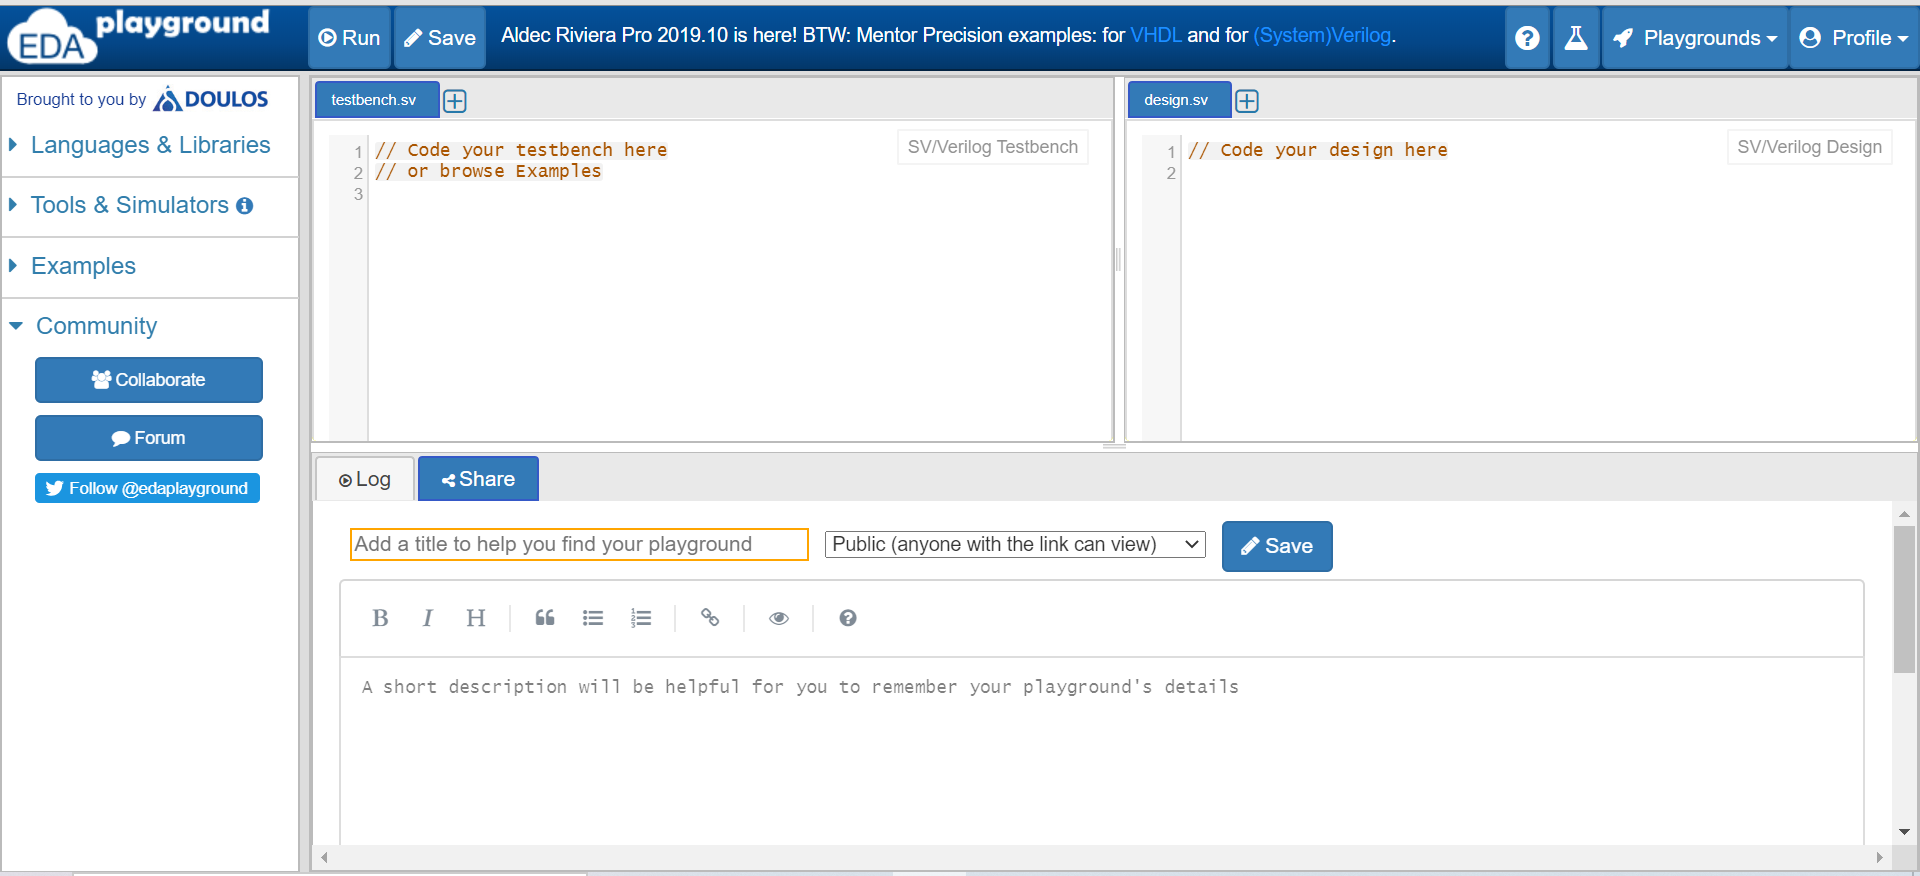
\includegraphics[width=0.75\columnwidth,height=4.5cm]{Figures/homeScreen.png}
            \label{fig: home}
        \end{figure}
    Your start-up screen after logging in should look like the above.    
    \item Click on \textbf{“Languages \& Libraries”}
    \item Select \textbf{“SystemVerilog/Verilog”} from \textbf{“Testbench + Design”}
    \item Click on \textbf{“Tools \& Simulators”}
    \item Select \textbf{“Icarus Verilog 0.10.0 11/23/14”} (All the Icarus Verilog options should work).
    Now you are set up to start coding.
    \item Copy and paste the testbench code below into the \textbf{“testbench.sv”} block.\\
    \textbf{Note}: In the testbench below, the clock is manually toggled before each operation. In more complex designs, it can be useful to use \verb|always| block to define the clock, and then just use regular wait designators between operations.
    
    \begin{Verilog}
    module ALU_tb();
    //inputs
    reg clk, A,B;
    reg[1:0] ALU_Sel;
    wire ALU_Out; // output
    
    //instantiate the module
     ALU ut(.clk(clk),
    .A(A),
    .B(B),
    .ALU_Sel(ALU_Sel),
    .ALU_out(ALU_Out)
    );

    initial begin

        $display("A  B  ALU_Sel  ALU_Out");
        $monitor("%b  %b  %b     %b",A,B,ALU_Sel, ALU_Out);
		
      	clk = 1'b1;
        A = 1'b1;
        B = 1'b1;
        ALU_Sel = 2'b0;
        #5
         clk=!clk;
      	#5
      	 clk=!clk;
      	 ALU_Sel = 2'b01;
        #5
         clk=!clk; 
         #5
      	clk=!clk;
       	ALU_Sel = 2'b10;
        #5
         clk=!clk;
        #5
      	 clk=!clk;
      	 ALU_Sel = 2'b11;
       #5
      	clk = !clk;
    end
endmodule
    \end{Verilog}
    
    \item In order to test different inputs, you can change the values of A and B. We'll test it with; \\
    1. A = 1'b0; B = 1'b1; \\
    2. A = 1'b1; B = 1'b0; \\
    3. A = 1'b0; B = 1'b0; 
    
   To do this, copy and paste the ALU code below into the \textbf{Design.sv block}
    
    \begin{Verilog}
   module ALU(
    input clk,A,B,
  	input [1:0] ALU_Sel,
    output reg ALU_out
);
  //output register
  reg ALU_Result;
    
  always@(posedge clk)
    begin
     case(ALU_Sel)
        2'b00: // Addition
           ALU_Result = A + B ; 
        2'b01: //Subtraction 
           ALU_Result = A - B;
        2'b10: //Subtraction
           ALU_Result = B - A;
        2'b11: //Multiplication
           ALU_Result = A * B;
        default: ALU_Result = A + B; //Addition
     endcase
    
     ALU_out <= ALU_Result;
    end
endmodule


    \end{Verilog}
    
    \item Click on \textbf{Save} in the top left corner and then \textbf{Run}.
    Your output (under log) should look like the following;
    \begin{figure}[H]
            \centering
            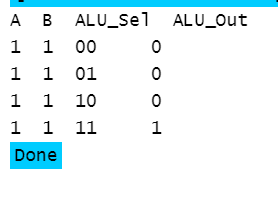
\includegraphics[width=0.25\columnwidth,height=3.5cm]{Figures/results.PNG}
            \label{fig: results}
        \end{figure}
    \item To display a waveform, click on \textbf{“Tools \& Simulators”}, click on the \textbf{“Open EPWave”} checkbox. Add the following lines of code in the testbench file in the initial block under monitor;
    
    \begin{Verilog}
        $dumpfile("dump.vcd"); 
      	$dumpvars;
    \end{Verilog}
    
    Save and Run
    
    \item The following simulation will pop up. To delete any of the fields, click on the name of the variable and click on the red x. To move a variable and wave up or down, click on the variable name and click on the up or down arrows. 
    After deleting and moving fields, a neatened simulation will look like this.
    
    \begin{figure}[H]
            \centering
            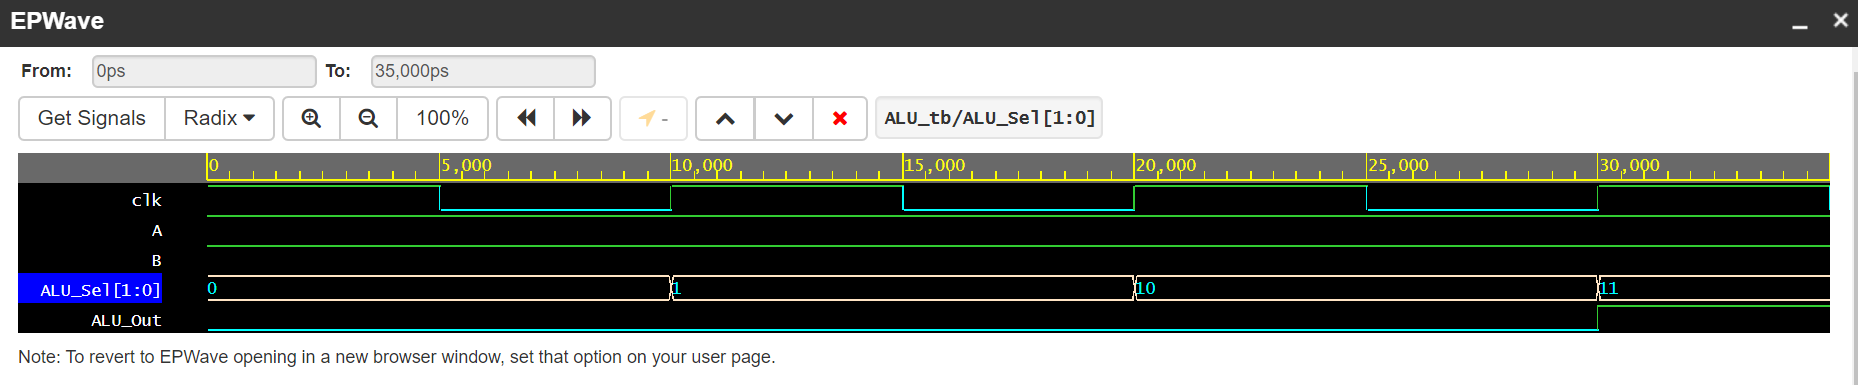
\includegraphics[width=1\columnwidth,height=4.5cm]{Figures/ALU_SIM.PNG}
            \label{fig: results}
    \end{figure}
    
    \item You can add your lab partner to collaborate on the same playgound as you. Go to \textbf{Community}, click on \textbf{Collaborate}. A block containing a link will pop up. Send this link to your partner who will then be able to edit the same playground as you. 
\end{enumerate}

% \subsection{ALU Questions}

% Answers to these questions need to be submitted in a single PDF to Vula.

% \begin{enumerate}
%     \item Consider a 4-bit ALU. Calculate the value of all four conditional flags (C, Z, N and V) after the following computations:
%     \begin{enumerate}
%         \item Let A = 0b0101, B = 0b0110 and the ALU performs an addition operation: S = A + B
%         \item Let A = 0b1000, B = 0b1111 and the ALU performs an addition operation: S = A + B 
%         \item Let A = 0b1000, B = 0b1111 and the ALU performs a subtraction operation: S = A - B 
%         \item Let A = 0b1000, B = 0b1111 and the ALU performs a subtraction operation: S = B - A 
%     \end{enumerate}
%     \item Design an arithmetic circuit for the ALU in table \ref{tbl:MiniALU}, which has a 3-bit instruction set. The opcodes in the instruction set are provided in the table below. Only design the system for the 1-bit case. You have the following components available to you: a single 1-bit full adder, 1-bit multiplexers, decoders, 1-bit flip flops and 2-input logical gates. An exclamation point (!) indicates the logical NOT operator.
% \end{enumerate}
% \begin{table}[H]
% \centering
% \caption{The instruction set for a mini ALU}
% \label{tbl:MiniALU}
% \begin{tabular}{|l|l|l|c|}
% \hline
% \textbf{S2} & \textbf{S1} & \textbf{S0} & \textbf{Operation} \\ \hline
% 0 & 0 & 0 & A + B \\ \hline
% 0 & 0 & 1 & A \\ \hline
% 0 & 1 & 0 & B - 1 \\ \hline
% 0 & 1 & 1 & A + !B \\ \hline
% 1 & 0 & 0 & A - !B \\ \hline
% 1 & 0 & 1 & A + 1 \\ \hline
% 1 & 1 & 0 & !B + 1 \\ \hline
% 1 & 1 & 1 & A - !B \\ \hline
% \end{tabular}
% \end{table}



\subsection{Questions}
Submit the following answers to Vula in a single PDF under the "tutorials" tab, correctly named.
\begin{enumerate}
    \item How do FPGAs differ from microcontrollers? Give two advantages of FPGAs, and 2 disadvantages. [2 marks]
    \item What is the difference between blocking and non-blocking assignments? Support your answer by comparing the two code snippets below and how their outputs may differ. [4 marks]
     \begin{figure}[H]
            \centering
            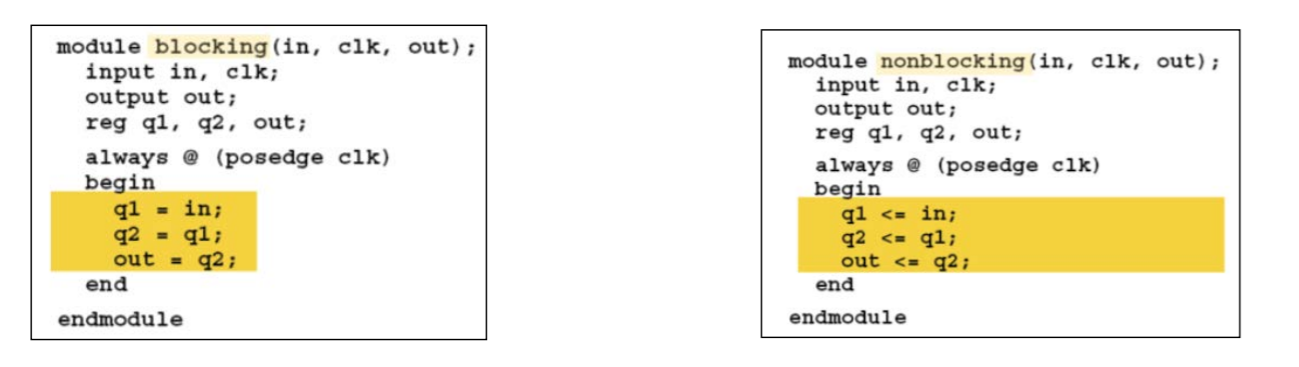
\includegraphics[width=1\columnwidth,height=4.5cm]{Figures/question 3.PNG}
            \label{fig: results}
    \end{figure}
    \item Port Mapping in module instantiation can be done in two different ways; \\
    1. Port Mapping by order\\
    2. Port Mapping by name
    
    \begin{Verilog}
module sum(
    input clk,A,B,
    output reg out
    );  
    always@(posedge clk)
    begin
	    out <= A+B;
    end
endmodule
    \end{Verilog}

For the module above; what is the output of the following testbenches done using port mapping by order (on the left) and mapping by name (on the right):
 \begin{figure}[H]
            \centering
            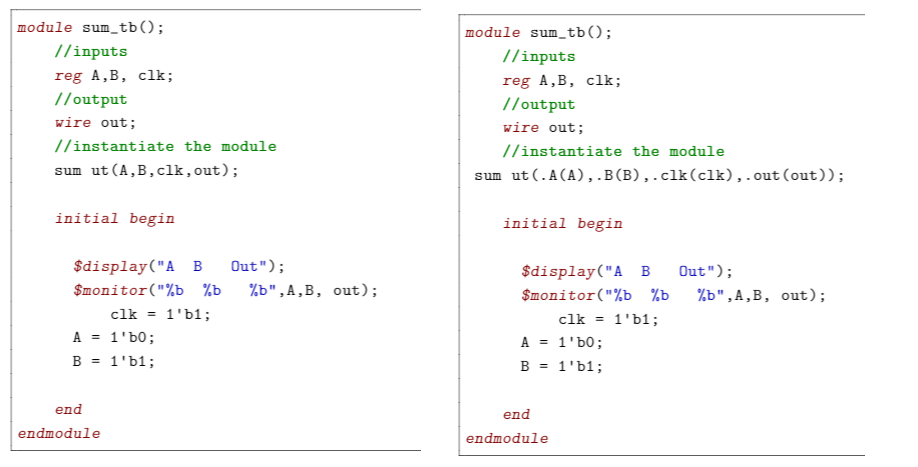
\includegraphics[width=1\columnwidth,height=6.5cm]{Figures/q4.PNG}
            \label{fig: results}
    \end{figure}

Comment on the results from each testbench. Which port mapping method is better to use when instantiating a module with many ports?  [2 marks]

\end{enumerate}

